La principale motivation dans le développement de couches morphologiques, initié à la fin des années 1980 \cite{Wilson_1989, Davidson_1990}, est l'intégration d'opérateurs morphologiques automatiques, capables d’apprendre et d’appliquer des érosions ou des dilatations sur des images données, au sein même des réseaux de neurones convolutionnels \cite{LeCun_2015}, en remplacement des couches de convolution classiques dans ces réseaux-ci. \\

\vspace{-1.4mm}
Ces nouvelles couches jouent ainsi, comme pour les couches classiques, le rôle de \textit{filtres} appliqués aux images en entrée du réseau, dont le noyau à poids variables est de taille constante, mais qui sont ici régis par une fonction particulière d'approximation de l'érosion et de la dilatation (approximation lisse nécessaire due à la non-dérivabilité du min et du max des opérations d'érosion et de dilatation). Le noyau de ces couches morphologiques joue alors un rôle analogue à celui des fonctions structurantes correspondantes, dont il cherche à imiter le comportement \cite{Bloch_2021}. Un réseau de neurones composé de telles couches est ainsi appelé << réseau de neurones morphologique >>. \\

\vspace{-1.4mm}
Soit $f: I \subseteq E \rightarrow \mathbb{R}$ une image, fonction sur une partie dénombrable $I$ de $E$ à valeurs dans $\mathbb{R}$, et soit $w: W \subseteq E \rightarrow \mathbb{R}$ le noyau d'une couche morphologique, également défini sur une partie dénombrable $W$ de $E$. Comme précédemment, on écrit $\breve{W}_x$ pour désigner l'ensemble symétrique de $W$ translaté de $x \in E$ :   $\breve{W}_x = \{ \, -\text{w} + x \, \mid \, \text{w} \in W \, \}$. \\

\vspace{-1.4mm}
\noindent \textbf{Attention} : Ici, nous parlons de << noyau >> ou de << filtre >> d'une couche pour désigner la fonction $w$ associée telle que définie ci-dessus et qui renvoie les poids $(w_y)_{y \in W} \in \mathbb{R}^{|W|}$ variables du filtre sur le support $W \subseteq E$. La << couche morphologique >>, quant à elle, est l'objet contenant à la fois ce noyau $w$ ainsi qu'une fonction de transformation $T$, qui prend en argument $w$ et qui, à partir d'une image $f$ en entrée de couche, renvoie une nouvelle image (également application de $I$ dans $\mathbb{R}$) en fonction de $f$ et $w$. \\


\vspace{-1.6mm}
\noindent D'une manière générale, la fonction de transformation $T$ peut être décomposée en deux étapes de transformations, l’une s'inscrivant dans l’autre. La première, locale, considère $f$ et $w$ localement en produisant, pour un point $x \in I$ donné, des \textit{familles de réels} à travers la mise en relation de la valeur $f(y)$ en $y \in \breve{W}_x$ avec la valeur $w(x-y)$ au point $x-y$ symétrique de $x+y$ par rapport à $x$. La seconde étape, plus globale, met en relation, pour ce même $x \in I$, l'ensemble des éléments de ces \textit{familles de réels} produites. Elle renvoie alors la valeur en ce point $x$ associée à la nouvelle image. Voir fig. \ref{fig:structure_couche_morpho}. \\

\vspace{-1.6mm}
\noindent Par exemple, pour une couche de convolution classique, la relation locale $\text{R}_\text{l}$ entre les $f(y)$ et $w(x-y)$ est le produit ($\times$), et la relation globale $\text{R}_\text{g}$ entre les éléments de la famille de réels produite est l'addition sur $y \in \breve{W}_x$. La nouvelle image $f_c$ issue de cette transformation $T$ est ainsi définie pour tout $x \in I$ par : $f_c(x) = \sum_{y \in \breve{W}_x} f(y) w(x-y)$. Pour une dilatation classique, $\text{R}_\text{l}$ est la somme (+), et $\text{R}_\text{g}$ est l'opération de maximum.
%D'une manière générale et plus informelle, la fonction de transformation $T$ d’une couche morphologique peut être décomposée en deux couches de transformation, qui s’imbriquent l’une dans l’autre. La première considère $f$ et $w$ de manière locale, et produit des familles de réels, pour un point variable $x$ donné, à travers la mise en relation de la valeur $f(y)$ de l'image $f$ en un pixel $y \in I$ avec la valeur $w(x-y)$ du noyau $w$ au pixel $x-y$ symétrique à $y$ par rapport à $x$, et ce pour tout $y \in \breve{W}_x$ créant ainsi une famille de réels indexée par $y \in \breve{W}_x$, et ce pour une ou plusieurs relations considérées. La seconde couche, plus globale, produit, à partir des éléments de ces familles de réels issus des relations entre $f(y)$ et $w(x-y)$ considérées pour un certain $x \in I$, la valeur au point $x$ associée à la nouvelle image. 
%Les relations locales entre les $f(y)$ et $w(x-y)$ n'apparaît pas explicitement dans la formule générale de $T$, mais deviennent explicites dans les différentes formules explicitées de $T$.



\newpage

% graphics
\begin{figure}[ht]
  \begin{center}
    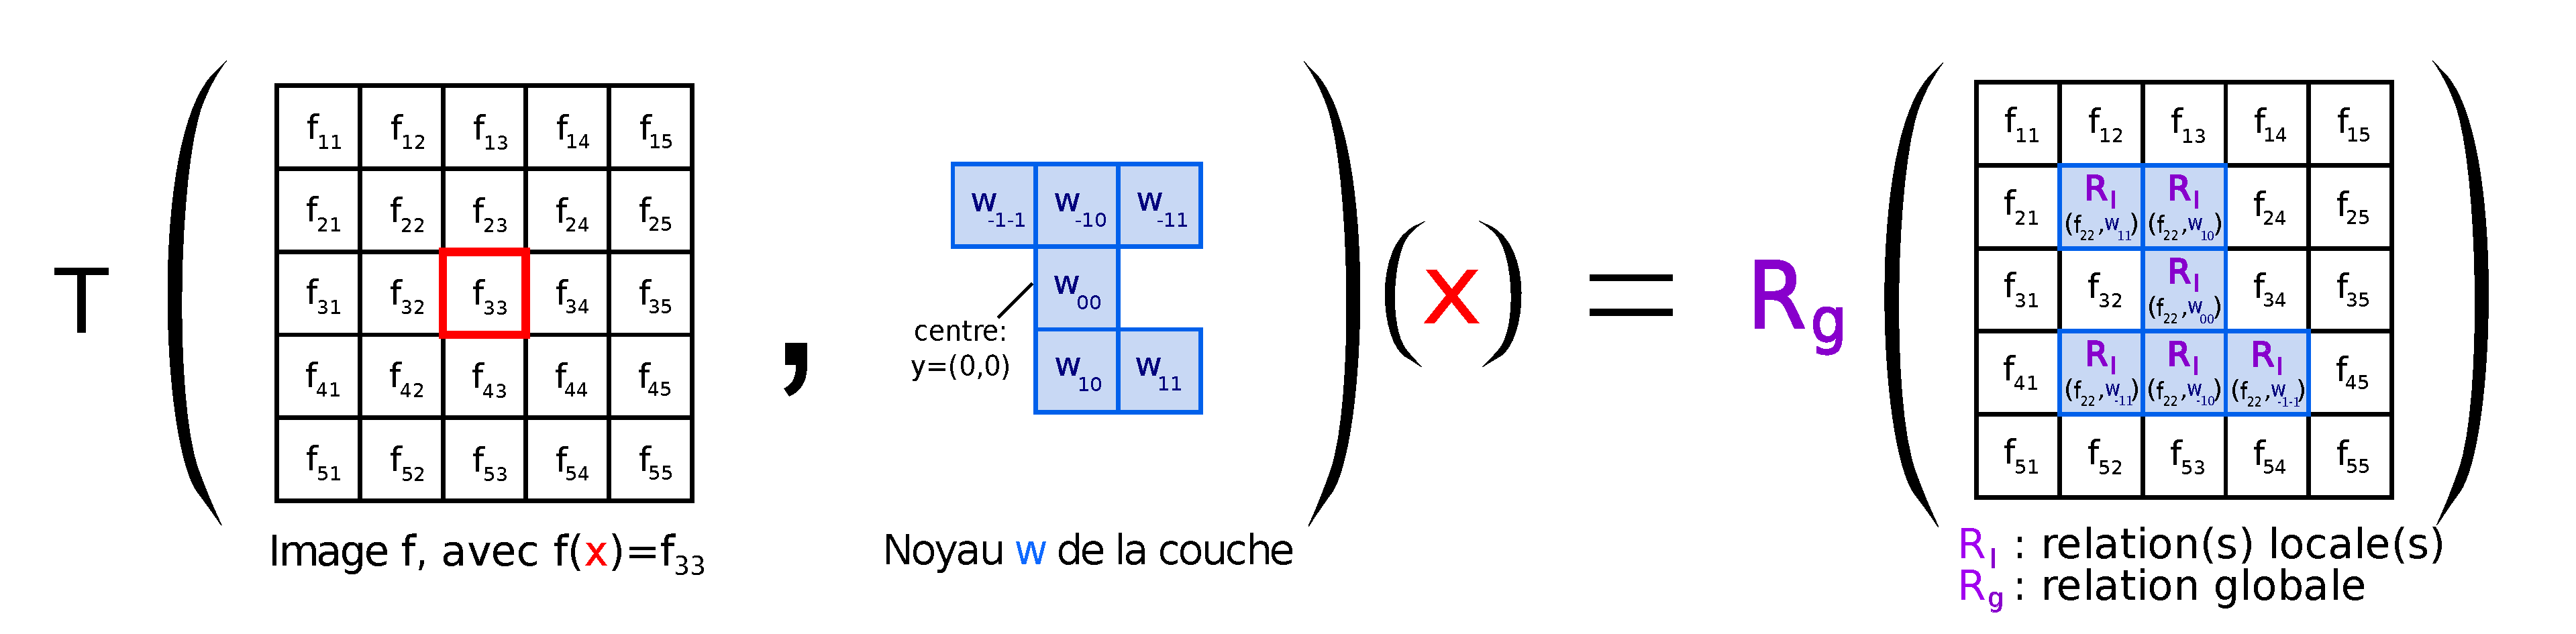
\includegraphics[width=1.00\textwidth]{parts/2-etat_de_lart/B-structure_des_reseaux_morphologiques/figures/couche_morpho.pdf}
    \caption{ \centering Illustration de la décomposition de la fonction de transformation $T$ en relations locales $R_l$ et une globale $R_g$, sur une image $f$ avec le noyau $w$ et au point $x$.}
    \label{fig:structure_couche_morpho}
  \end{center}
\end{figure}

\vspace{-1.8mm}
\noindent La fonction $T$ renvoie l'image $T(f,w)$ définie sur $I$ dans $\mathbb{R}$. On écrira cette nouvelle image, sans expliciter les relations locales $\text{R}_\text{l}$ entre les $f(y)$ et $w(x-y)$ ou globale $\text{R}_\text{g}$, simplement comme suit :
\vspace{-2.6mm}
\begin{align*}
T(f,w) \colon I & \longrightarrow \mathbb{R}\\
x & \longmapsto T \left ( f, w \right ) (x)
\end{align*}

\vspace{1.0mm}
\noindent La fonction de transformation $T$, qui prend en argument le couple image-noyau $(f,w)$, transforme ainsi l'image $f$, en entrée de la couche, en une nouvelle image de même taille, en considérant, pour chacun des pixels $x$ appartenant au support $I$ de l'image d'entrée, le voisinage défini par le support $W \subseteq E$ du noyau $w$ (illustration fig. \ref{fig:structure_couche_morpho}). \\

La bonne définition d'une telle fonction de tranformation $T$ au sein d'une couche permettrait d'appliquer à l'image $f$ l'effet désiré (convolution, max-pooling, morphologie, etc.), avec les poids du noyau $w$ de la couche en question, grâce à des mises en relation locales entre $f(y)$ et $w(x-y)$ et à une relation globale sur toutes ces dernières. \\

\vspace{-1.6mm}
\noindent Dans le cadre des réseaux de neurones, on va définir ces différentes relations de sorte que la fonction $T$ soit \textit{continue} et \textit{dérivable} localement partout par rapport aux poids $(w_y)_{y \in W}$ variables du noyau $w$, afin de pouvoir calculer le gradient du réseau lors de la phase d'apprentissage et mettre à jour ces poids par rétropropagation du gradient. \\

Le but ici, dans le cadre des couches morphologiques, est alors de trouver une fonction dérivable $T$ (et donc de définir les différentes relations locales et globale telles que décrites ci-dessus) adaptée, pour approximer au mieux l'effet des deux opérateurs morphologiques fondamentaux, l'érosion et la dilatation, et ce en une \textit{unique} formule. \\

\vspace{-1.6mm}
\noindent Ici, les noyaux des couches morphologiques seront toujours accompagnés d'un poids supplémentaire, noté $p$ ou $\alpha$, qui est indépendant des poids du noyau-même, et dont le rôle sera de faire une transition continue lisse entre le comportement d'érosion et celui de dilatation de la couche morphologique \cite{Hermary_2022}. Pour mieux distinguer ce poids des autres, on notera la nouvelle image de $T$: $T(f,w,p)$. Les différentes définitions de la fonction de transformation $T$ et l'intégration du poids $p$ sont explicitées partie 2.3.
